\documentclass[runningheads]{llncs}

\usepackage[backend=biber]{biblatex}
\bibliography{AGI-book}

\usepackage[T1]{fontenc}
% T1 fonts will be used to generate the final print and online PDFs,
% so please use T1 fonts in your manuscript whenever possible.
% Other font encondings may result in incorrect characters.
%
\usepackage{graphicx}
% Used for displaying a sample figure. If possible, figure files should
% be included in EPS format.
%
% If you use the hyperref package, please uncomment the following two lines
% to display URLs in blue roman font according to Springer's eBook style:
%\usepackage{color}
%\renewcommand\UrlFont{\color{blue}\rmfamily}

\usepackage{amsmath}
\usepackage{amssymb}    % for \rightsquigarrow
\usepackage{wasysym}	% for frown face
\usepackage{mathrsfs} 	% for \mathscr
\usepackage{stmaryrd}
\usepackage{mathtools}		% to extend length of double harpoon arrows

\begin{document}
%
\title{AGI from the perspectives of Categorical Logic and Algebraic Geometry}
%
%\titlerunning{Abbreviated paper title}
% If the paper title is too long for the running head, you can set
% an abbreviated paper title here
%
\author{King-Yin Yan \orcidID{0009-0007-8238-2442}}
%
\authorrunning{K-Y. Yan}
% First names are abbreviated in the running head.
% If there are more than two authors, 'et al.' is used.
%
\institute{\email{general.intelligence@gmail.com}}
%
\maketitle              % typeset the header of the contribution
%
\begin{abstract}
To ``situate'' AGI in the context of some current mathematics, so that readers can more easily see whether certain mathematical ideas can be fruitfully applied to AGI.

\keywords{AGI  \and categorical logic \and homotopy type theory  \and algebraic geometry \and topos theory \and neural-symbolic integration}
\end{abstract}
%
%
%
\section{Goal of this paper}

The bottleneck of AGI development is the speed of learning algorithms.  The daily cost of running GPT-4 was rumored to be \$700K by Sam Altman.  To speed up learning, one needs \textbf{inductive biases}, according to the \textbf{No Free Lunch theorem} \cite{Wolpert1997} \cite{Wikipedia-no-free-lunch}.  A principled way to introduce inductive bias is by the structure of logic. 
% Traditionally this line of research is called algebraic logic, starting from Leibniz and Boole, up to more recent times Tarski's cylindrical algebra and Paul Halmos' work.  

\section{Results thus far}

Most of the ideas in this paper are not yet ready to offer practical ways to accelerate AGI.  Nevertheless the author hopes it can help readers on their way to discover more ingenious ideas.

In each section below, we look at one aspect of the categorical structure of logic and speculate on how it might aid AGI architecture.

\subsection{Where is GPT?}

\begin{figure}
	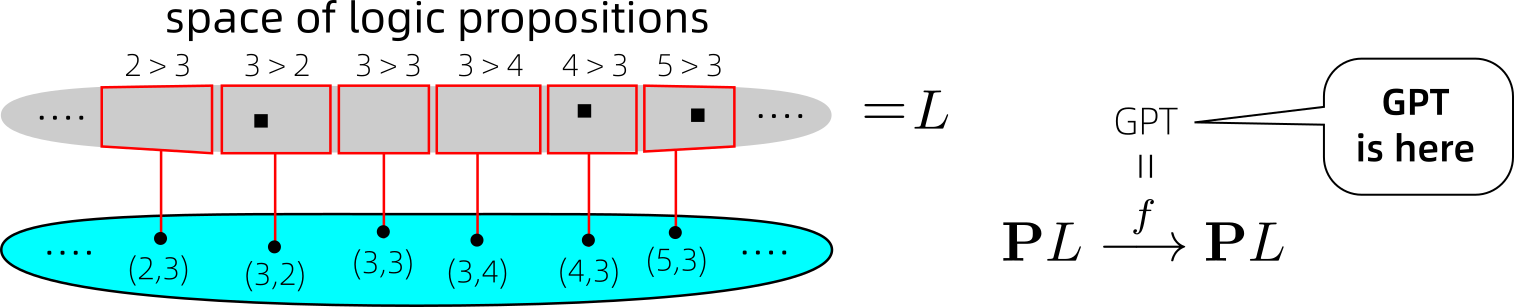
\includegraphics[scale=.5]{GPT-is-here.png}
	\caption{(Left) A sheaf of propositions over pairs of natural numbers; (Right) The function space where GPT lives. $\wp(L) = 2^L$ is the power set of $L$.}
	\label{fig:GPT-is-here}
\end{figure}

GPT \cite{chatGPT2020} can be regarded as a \textbf{logic consequence operator} mapping from the space of propositions to itself (as a \textbf{set-valued map} \cite{Aubin1990}), as shown in Fig.\ref{fig:GPT-is-here}.

\begin{figure}
	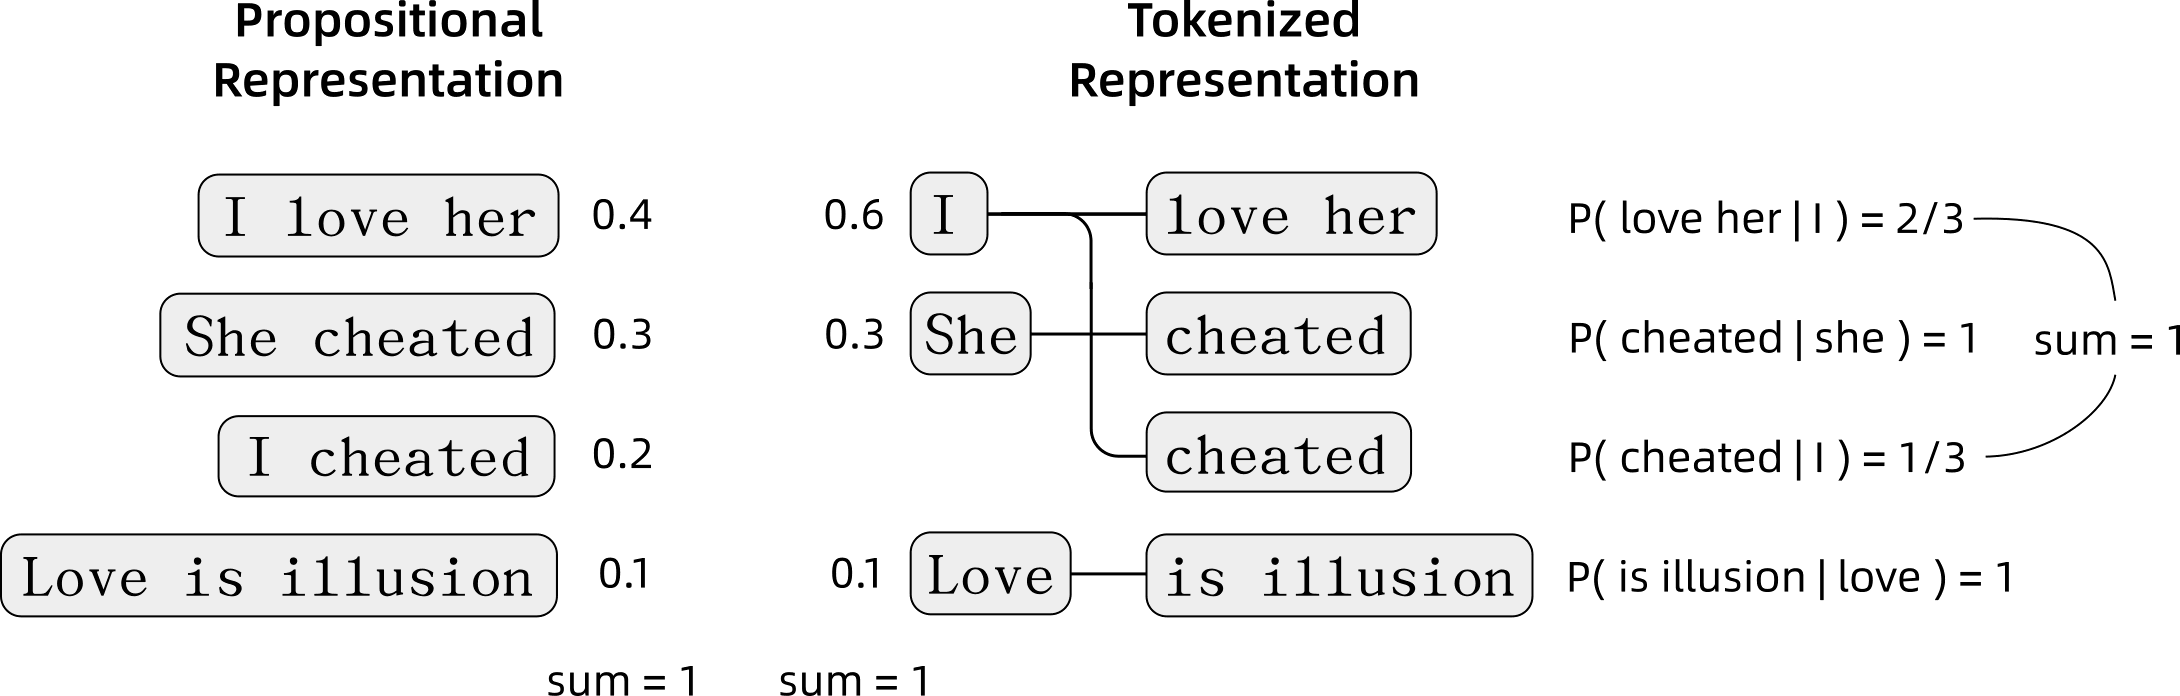
\includegraphics[scale=.4]{I-love-her-she-cheats.png}	% width=\textwidth
	\caption{The equivalence of probability distributions over propositions and over tokens. For simplicity the decomposition for just the leading token is shown.} \label{fig:she-is-bitch}
\end{figure}

Without loss of generality, GPT can be seen as acting on propositions, as probability distributions on tokens are equivalent to probability distributions on sentences (propositions), see Fig. \ref{fig:she-is-bitch}.

To what extent can we say that GPT output vectors live in a Curry-Howard type-theoretic space?  A neural network (eg. GPT) always maps an input to the the same output vector, as it is a \textit{deterministic} map. Thus it seems meaningless to ask what is the meaning of the \textit{neighborhood} of an output vector, if the network never goes there during inference time.

\begin{figure}
	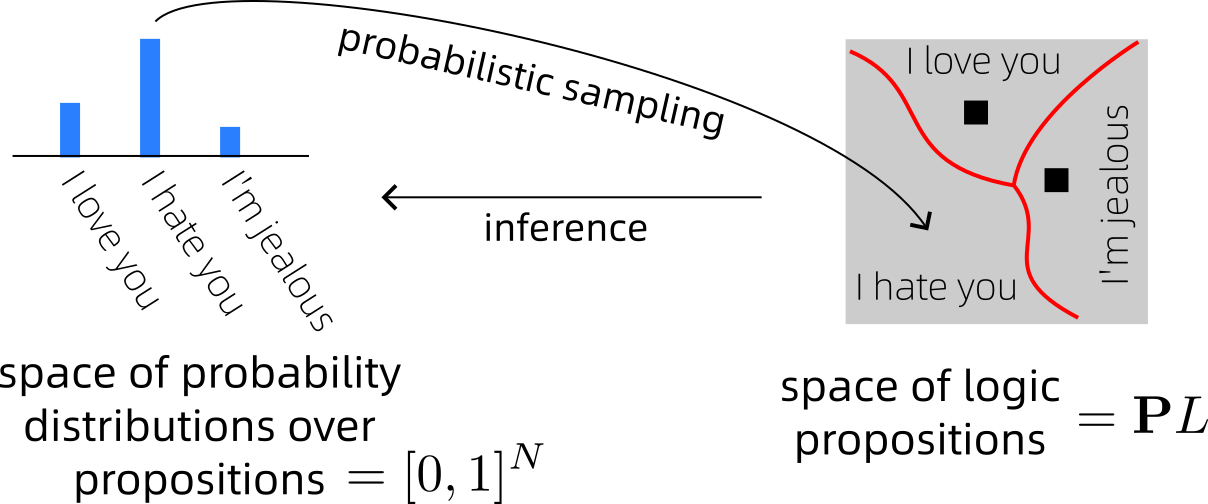
\includegraphics[scale=.45]{Transformer-output.png} \quad
	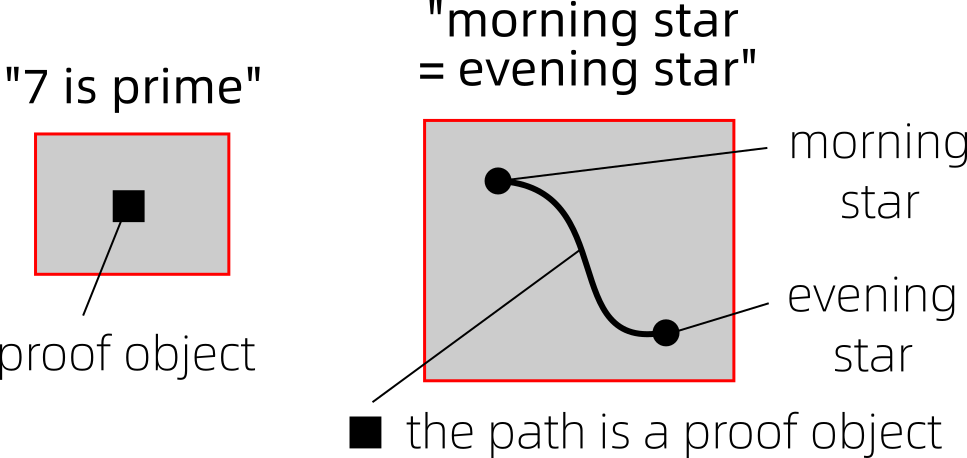
\includegraphics[scale=.35]{morning-star.png}
	\caption{(Left) The GPT or Transformer outputs a continuous-valued vector which is interpreted as a probability distribution over tokens, which is then sampled to output a specific token, such as `hate' or sequentially an entire proposition such as `I hate you.'  These tokens are discrete symbols that always map to the same vector-embedding positions.  Thus, during inference, an input vector will not 'wriggle' near some neighborhood; it is either at one vector position or it jumps to another position.  Thus the inference ``paths'' inside GPT layers are always fixed, once learning has finished.  $N$ = size of vocabulary or sentences; (Right) In HoTT, a path is a proof object of an \textbf{identity type}.}
	\label{fig:morning-star}
\end{figure}

Fig.\ref{fig:morning-star}(Left) illustrates why even despite probabilistic sampling, the outputs of GPT seem to follow fixed trajectories (during inference time).  Nevertheless, if we artificially ``perturb'' the input, the output probability distribution will change \textit{smoothly}, say from favoring token $A$ to favoring token $B$, as neural networks are always \textit{differentiable} functions.  One can define the \textbf{boundary} between tokens $A$ and $B$ as where their probabilities reverse in magnitude.  This forms a Voronoi-like tessellation of the output space that can be regarded as Curry-Howard type-spaces.

\subsection{Homotopy type theory (HoTT)}

HoTT is a step along the Curry-Howard tradition where propositions = types = topological spaces, and such spaces are given \textbf{homotopy} structure.  An example is ``morning star = evening star'', illustrated in Fig.\ref{fig:morning-star}(Right).  But the enterprise does not end here: higher homotopy types give rise to a hierarchy up to $\infty$-groupoids.  From my shallow understanding of this subject, this seems to suggest that proofs have their own proofs, so that an entire \textbf{inference trace} can be recorded as homotopy paths.  Having inference traces recorded may be useful from the perspective of \textbf{Truth Maintenance Systems}\footnote{TMSs are systems that enhance rule-based problem solvers by providing the ability to make default assumptions, recover from inconsistencies, etc; functions that are beyond the scope of simple logic-based systems.  They are closely related to belief revision and paraconsistency.  See \cite{wikiTMS} for more.} of classical AI.

From the previous section we may argue that the output vectors of a neural network can be regarded as \textbf{proof objects} in their respective type-spaces.  However we can also argue that such type-spaces as implemented by neural networks are \textit{unlikely} to have complex internal structures, because one proof object must vary \textit{smoothly} into another proof object.  To be able to process HoTT information, we may need neural networks with \textbf{fractal structure} (ie, it can recognize vectors belonging to a fractal pattern, such as a Cantor set.  This can be implemented programmatically using recursion + scaling), but current neural architectures seem to lack it.

\subsection{Commutativity of $\wedge$ and $\vee$}

Permutation symmetry is the easiest to recognize and implement \cite{Zaheer2017} \cite{Qi2017}.  It is well-known the Transformer \cite{Vaswani2017} is \textbf{equivariant} to permutations of inputs.  This may be seen as evidence that Transformer \textbf{tokens} are proposition-like entities, whose Boolean algebra has $a \wedge b = b \wedge a$.  But we need to be cautious of confusing the propositional level with the sub-propositional level of words or atoms.  In standard predicate logic, $\heartsuit(a,b) \neq \heartsuit(b,a)$.  The Transformer may handle this as a sequence of tokens like ``$a , \heartsuit , b$'' which is not the same as ``$b , \heartsuit , a$.''  This reminds us that Transformers need to use \textbf{positional encoding} at the input layer, when word order is important.

\subsection{$\forall$ and $\exists$ as adjunctions}

It seems difficult to translate this structure into a structural modification of neural networks.  From our experience in logic-based AI, logic rules are usually implicitly $\forall$-quantified, and $\exists$ is usually implicit by the \textbf{Closed-World Assumption}.

The following two conditions concern the well-behavior of quantification, as described in \cite{Jacobs1999} and on nLab \cite{nLab-beck-chevalley} \cite{nLab-Frobenius}:

\noindent The \textbf{Beck-Chevalley condition} says that substitution of free variables commutes with quantification.

\noindent The \textbf{Frobenius condition} corresponds in logic to saying that $\exists x. (\phi \wedge \psi)$ is equivalent to $(\exists x. \phi) \wedge \psi$ if $x$ is not free in $\psi$.

Both conditions are ``self-evident'' from the logic perspective, but it remains to be seen how they can be applied to neural networks.

\subsection{Predicates as fibration}

The relevant mental picture here is Fig.\ref{fig:GPT-is-here}(Left). Current neural networks seem to operate in the space $L$ above the base space and are unaware of the predicate-fibration structure.  Knowledge graphs have an obvious \textbf{first-order structure} as they are made of nodes and links.  One can embed nodes into a metric space $D$ and form the Cartesian product $D \times D$, then a link $a\,R\,b$ is just a point sitting vertically above this domain, and the relation $R$ is a point-set or its \textbf{cover}.  This setup may increase efficiency if we know \textit{a priori} that the dataset is first-order.

More interesting is the case of \textbf{higher-order logic} (HOL), which means we can have quantified rules \textit{over} relations, which suggests we should embed rules in the same manner as we embedded first-order objects.  This seems to require, again, the use of \textbf{set-valued maps}.

\subsection{Iteration of $\vdash$ and Looped Transformers}

This idea is easy to implement, and it also comes from an obvious feature of logic:  we know that inferences in logic are \textit{repeated} applications of the \textit{same} set of rules of a knowledge-base $K$, $\Gamma \vdash_K \vdash_K ... \vdash_K \Delta$.  But current Transformer architectures (which can be > 100 layers deep) do not re-use their layers at a fine scale.  Perhaps the recent research in \textbf{Looped Transformers} \cite{Yang2024} \cite{Giannou2023} can offer improvements in this direction.

\subsection{Modal logic}

\begin{figure}
	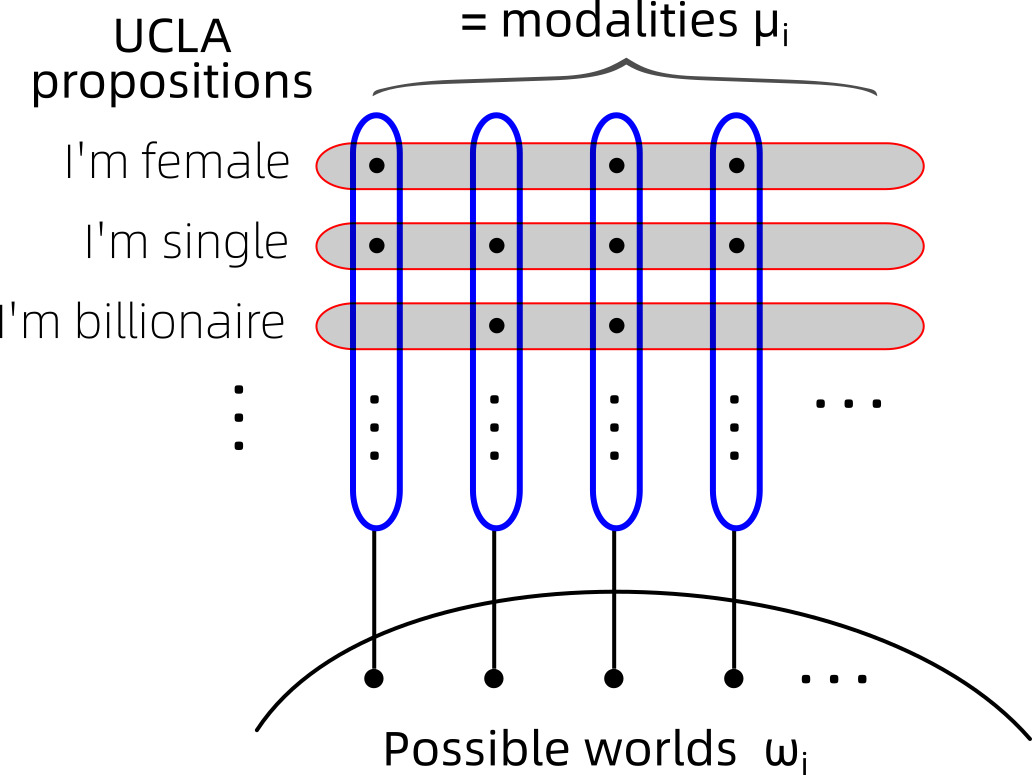
\includegraphics[scale=.5]{possible-worlds-as-sheaf.png} \qquad
	\raisebox{.5cm}{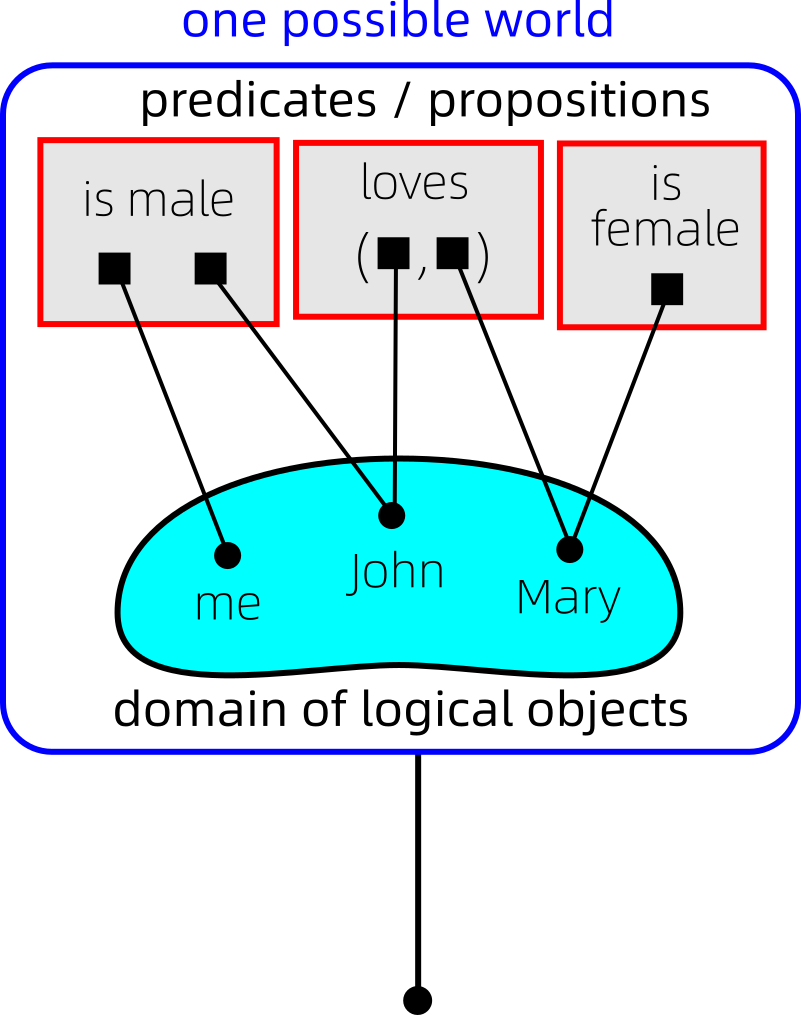
\includegraphics[scale=.35]{possible-world-single-example.png}}
	\caption{(Left) The space underneath are possible worlds, where each world is an \textbf{open set}. Each \textbf{stalk} above represents the propositions true in that world, together they form a \textbf{fibration} over the base space. (Right) The \textbf{structure} for interpreting \textbf{first-order} logic in one world.}
	\label{fig:possible-worlds-as-sheaf}
\end{figure}

Modal logic \cite{Goble2001} \cite{Popkorn1994} may be useful in AGI for dealing with various ``modalities'' such as knowledge, obligations, time, intension, etc.  Special to modal logic are the operators $\Box$ (\textbf{necessity}) and $\Diamond$ (\textbf{possibility}).  Syntactically it is obvious that $\Box \Box A \equiv \Box A$, and Tarski-McKinsey (1944) cf. \cite{Dunn2001} discovered that $\Box$ and $\Diamond$ can be interpreted by the \textit{topological} operations of \textbf{interior} and \textbf{closure} respectively.  % The interior $\mathrm{Int} A$ is defined as the union of all open sets in $A$.  
% If $\Box A = \mathrm{Int} A =$ Universe then $\Box A$ is interpreted as true.  For example in Fig.\ref{fig:possible-worlds-as-sheaf}(Left) ``I'm single'' is true in all possible worlds, so it can be concluded to be \textit{necessarily} true.  % 
One could say \textbf{Grothendieck topology} is re-captured as a modal operator in the logic setting \cite{Rodin2014} \S5.9.

Fig.\ref{fig:possible-worlds-as-sheaf}(Left) is the setup for \textbf{sheaf semantics} \cite{Goldblatt1984} \cite{Bell1988}, for interpreting \textbf{propositional} modal logic.   On the right is the \textbf{structure} for interpreting \textbf{first-order logic} in a single possible world, which contains a \textbf{domain} for interpreting predicates, relations, and functions.  These two can be combined to interpret \textbf{first-order modal} logic \cite{Awodey2007} \cite{Awodey2014}. The resulting structure is called a \textbf{comma category} \cite{MacLane1997} or \textbf{slice category} and can be denoted $\mathbf{Sets}/K$ where $K$ is the set of worlds.

Every sheaf automatically admits a \textbf{Yoneda embedding}\footnote{The Yoneda lemma can be understood as saying some object in a category is able to ``represent'' the entire category.  A archetypal example is \textbf{Cayley's theorem} in group theory, that says that every finite group is isomorphic to a subgroup of the symmetric group $\mathfrak{S}_n$. Here the symmetric group is the \textbf{representing object} capable of representing all finite groups.}.  In this case the representation seems to involve the notion of \textbf{UCLA propositions} \cite{Dunn2001} (named after researchers from the University of California) which defines a proposition as \textit{equivalent} to the \textbf{set} of possible worlds in which it is true. The truth-value object $\Omega$ for a pre-sheaf category is itself a pre-sheaf (because it has to be an object of the category in question), and in particular it is a set of sieves over base objects.  

Modal logic is also useful for interpreting \textbf{intensional logic} \cite{Stanford2022-intension}.  For example, ``the tallest building in New York'' is a term that can \textbf{designate} different buildings at different times (worlds), which requires a \textbf{function} to map the term to different objects at different worlds.  Such functions exist in the structure in Fig.\ref{fig:possible-worlds-as-sheaf}(Right).

In practice, however, the possible worlds we can handle may be just a \textbf{discrete} set with few elements (think of how many \textit{chess moves} you can calculate in your head, each move being one possible world).  %$\mathrm{Int} A$ of a discrete set is just $A$ itself.

The worlds being \textbf{open sets}, which are idealized objects, is difficult to implement on a computer.  However note that such sets are \textbf{overlapping} as shown in Fig.\ref{fig:possible-worlds-as-sheaf}(Left), and their embedding in \textbf{metric} space is perhaps more meaningful and of practical value.  Alternatively they can be processed \textbf{syntactically} by rules of modal logic, which might have occurred to a certain degree in current Large Language Models (LLMs).

\subsection{Algebraic geometry and topos theory}

The fundamental duality in algebraic geometry is:
\begin{equation}
\left\{ \begin{tabular}{cc} spaces, or \\ varieties \end{tabular} \right\} \longleftrightarrow \left\{ \begin{tabular}{cc} commutative \\ $\mathbf{k}$-algebras \end{tabular} \right\}
\end{equation}
within this correspondence, ``points'' in geometry are identified with \textbf{prime ideals}.
%\begin{equation}
%\left\{ \begin{tabular}{cc} points in \\ geometry \end{tabular} \right\} \longleftrightarrow \left\{ \begin{tabular}{cc} prime ideals \end{tabular} \right\}
%\end{equation}

An approach suggested by Yuri Manin \cite{Manin2009} \cite{Manin2018} \S1.1.3d is to turn logic into an \textbf{algebra}, such as the Boolean ring (but this can only handle propositional logic).  Varieties defined by such Boolean polynomials \cite{Lundqvist2015} live in the space $\mathbb{Z}_2^n$, the \textbf{discrete hypercube}.  

The \textbf{algebraization} of logic is a subject with a long history that dates back to Leibniz and George Boole, with more recent names like Tarski, Rasiowa, Sikorski (they're Polish), Paul Halmos \cite{Halmos1962} \cite{Halmos1998}, Don Monk \cite{Monk1971}, the Hungarians Hajnal Andr\'{e}ka and Istv\'{a}n N\'{e}meti \cite{Andreka1991} \cite{Andreka2021}.  

One can push Grothendieck's algebraic geometry to its limit, with the slogan ``logic is geometry controlled by set theory'', but this seems to be a \textit{separate} path from the Curry-Howard-categorical tradition.  Anyway, we now turn to the latter.

%My visualization of the ``Grothendieck picture'' of AGI is like this:
%\begin{equation}
%\vcenter{\hbox{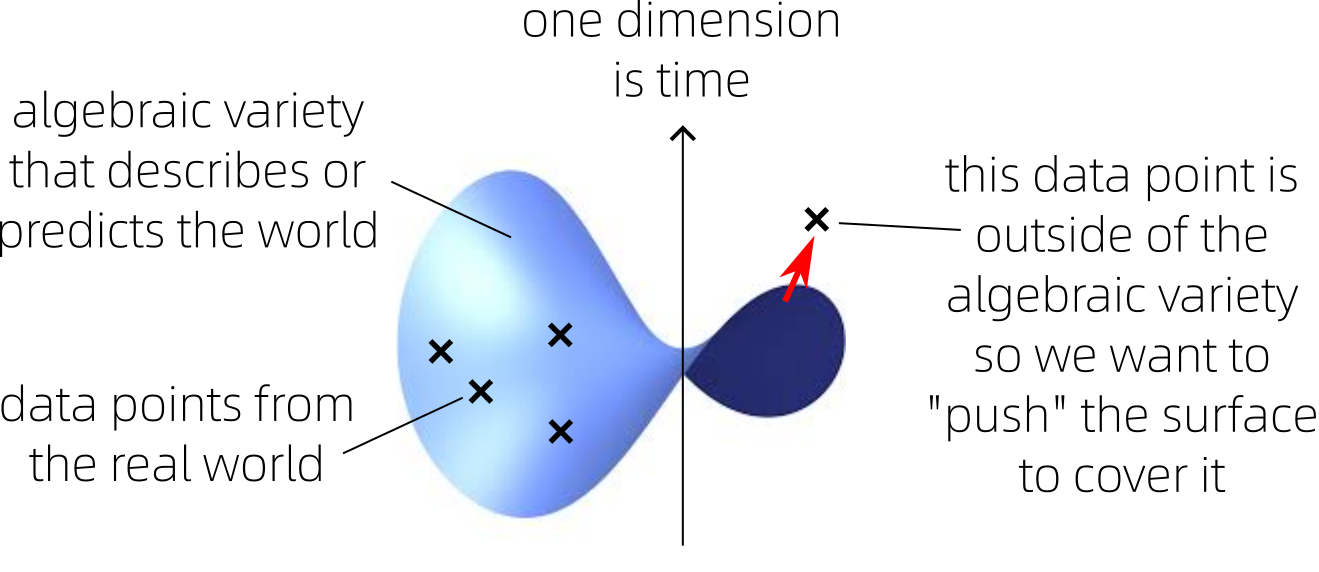
\includegraphics[scale=0.4]{Grothendieck-picture.png}}} \nonumber
%\end{equation}

One of the interesting discoveries in categorical logic is that every topos admits an \textbf{internal language}.  This is a simple consequence of Curry-Howard: since a type-space corresponds to a logic proposition, and categorical logic interprets type-spaces as objects in a category, thus every category (satisfying extra conditions) can be interpreted as having an ``internal'' logic.  The converse of this correspondence is the \textbf{classifying topos} of a logic theory $\mathbb{T}$:
\begin{equation}
\underset{\footnotesize\text{classifying topos}}{\mathcal{E}_\mathbb{T}} \xrightleftharpoons[]{\; \text{ internal language } \;} \underset{\footnotesize\text{theory}}{\mathbb{T}}
\end{equation}

Olivia Caramello \cite{Caramello2018} developed an idea where toposes play the central role of ``bridges'' that transfer information between theories (AGI can be seen as the \textbf{common-sense theory} of our physical world).  She showed that for any geometric theory $\mathbb{T}$, interpreted in the Grothendieck topos $\mathcal{E}_\mathbb{T}$, there is a \textbf{universal} model $U$ such that any model of $\mathbb{T}$ up to isomorphism is a pullback of $U$ along a geometric morphism.  This means that the \textbf{classifying topos} of $\mathbb{T}$ is the \textbf{representing object} in a \textbf{Yoneda embedding}.  A diagram in her book is reproduced here with simplifications in Fig.\ref{fig:Caramello-pic}(Left).

\begin{figure}
	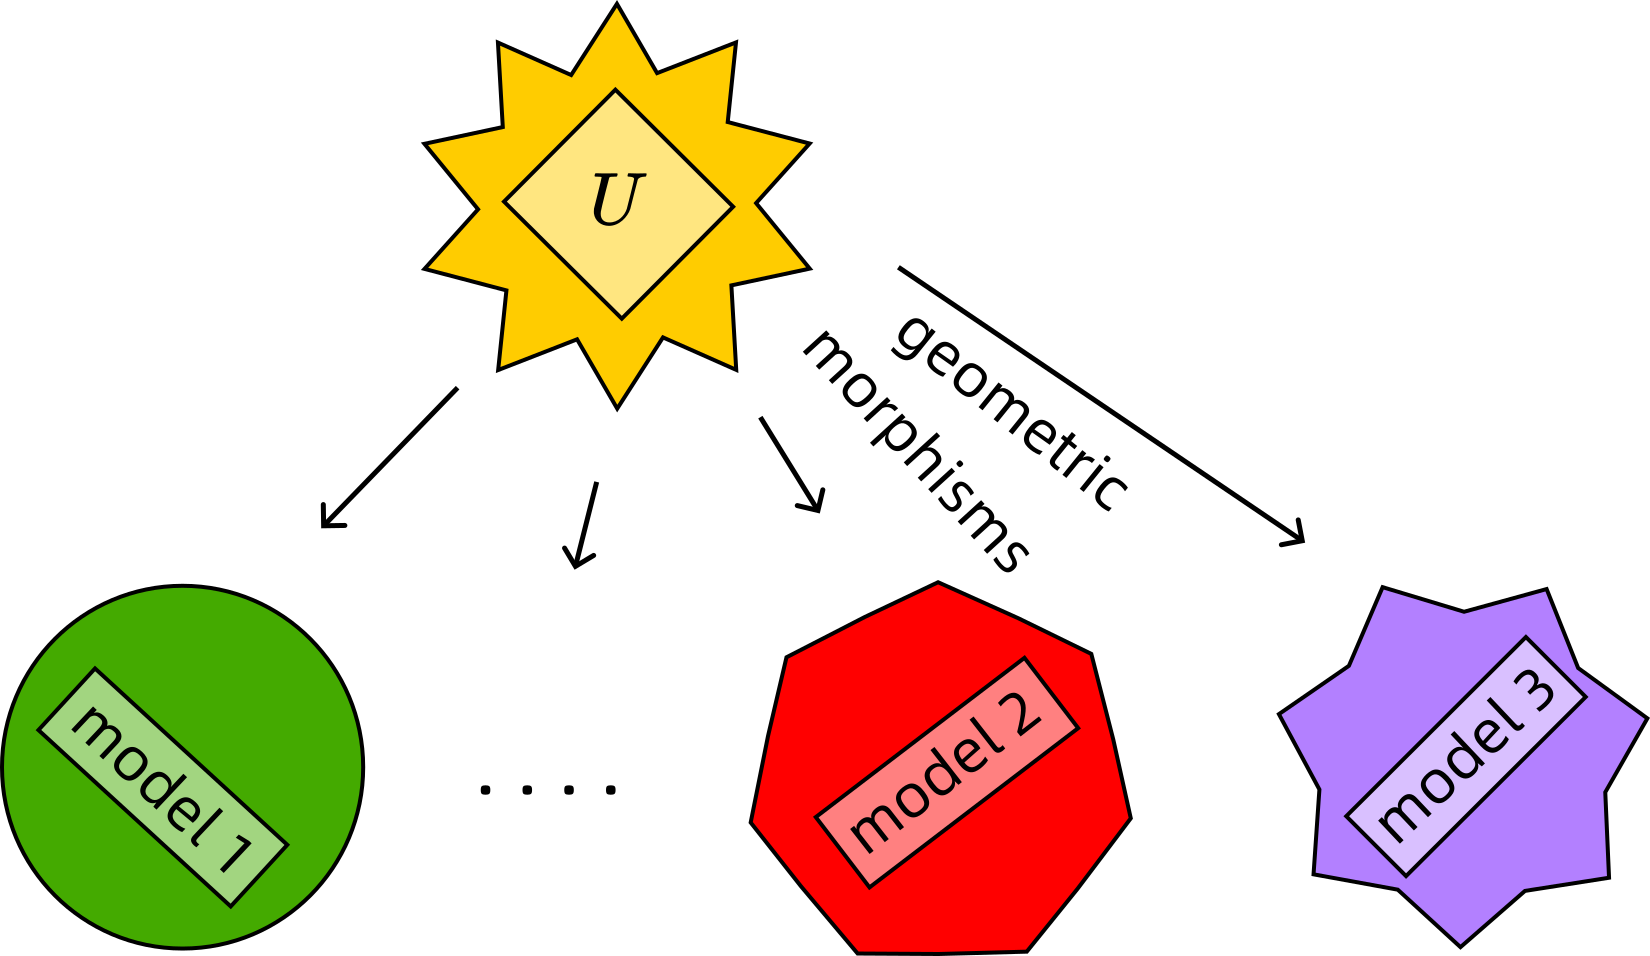
\includegraphics[scale=.25]{Caramello-picture.png} \qquad
	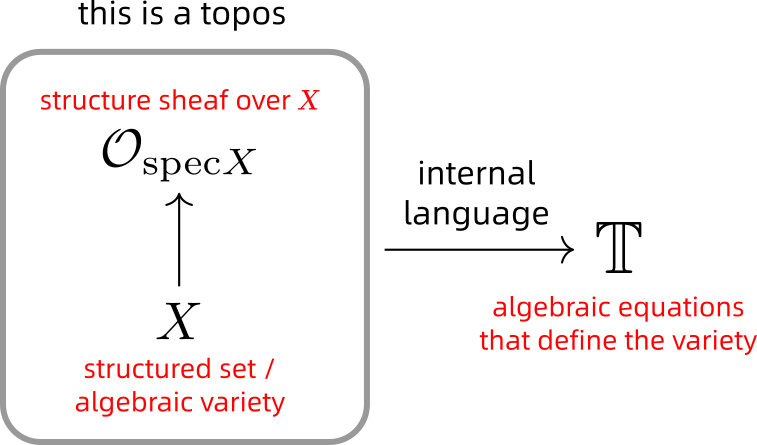
\includegraphics[scale=.5]{geometric-topos.png}
	\caption{(Left) The universal model $U$ sits inside its classifying topos (darker color); (Right) The classical formulation of algebraic geometry}
	\label{fig:Caramello-pic}
\end{figure}

In a similar vein, Ingo Blechschmidt's PhD thesis \cite{Blechschmidt2017} and his IHES presentation 9 years ago \cite{Blechschmidt-video2015} brings the categorical idea of internal language back to its classical setting in algebraic geometry.  The situation is as depicted in Fig.\ref{fig:Caramello-pic}(Right).  In this setup, the internal logic comes from the (``big'' and ``small'') \textbf{Zariski topology} of the base space, or \textbf{site}.  The basic idea is that the topology of \textbf{open sets} is a \textbf{Heyting algebra} that can be interpreted as \textbf{intuitionistic logic}\footnote{\textbf{Negation} is interpreted by the \textbf{interior} of the complement so as to have open sets all the way.  This leaves the boundary out, thus $A \vee \neg A =$ Universe is not generally valid, as opposed to classical logic.}.  The external view of ``sheaves of objects'' is simplified to ``plain objects'' in the internal view, where such objects can be rings (such as $\mathcal{O}_{\mathrm{spec} X}$), modules, etc.  The ring $\mathcal{O}_{\mathrm{spec} X}$ contains the polynomials that define the algebraic variety $X$, and the internal logic can be used to reason about such polynomials.

Andrei Rodin in his book \cite{Rodin2014} argues that logic is an axiomatic \textbf{abstraction} of the objective world, or as Lawvere puts it, we should ``\textit{concentrate the essence of practice to guide practice}'' (in the Foreword to \cite{Adamek2011}).  This serves as a nice closing remark.

% Grothendieck 的方法是透过抽象,将技巧转移到新的范围....  但有没有可能将几何的技巧应用在自然语言逻辑? 

% 代数几何中最特别的地方是出现了 由代数方程 =0 定义的代数簇,这个带结构的空间 与抽象的 scheme 对应,scheme 是研究代数簇的更抽象而合理的对象。 范畴逻辑来自 Curry-Howard 的传统,我研究的目的是寻找 逻辑在数学中的适当位置,但也寻找逻辑的更 general 形式。 逻辑加入了「数量」运算之后,可以处理「方程」的问题,而在另一方向发展,它处理自然语言的问题。

%
% ---- Bibliography ----
%
% BibTeX users should specify bibliography style 'splncs04'.
% References will then be sorted and formatted in the correct style.
%
% \bibliographystyle{splncs04}
\printbibliography

\end{document}
